\documentclass[onecolumn]{article}
\usepackage{url}
\usepackage{algorithmic}
\usepackage[a4paper]{geometry}
\usepackage{datetime}
\usepackage[margin=2em, font=small,labelfont=it]{caption}
\usepackage{graphicx}
\usepackage{mathpazo} % use palatino
\usepackage[scaled]{helvet} % helvetica
\usepackage{microtype}
\usepackage{amsmath}
\usepackage{subfigure}
% Letterspacing macros
\newcommand{\spacecaps}[1]{\textls[200]{\MakeUppercase{#1}}}
\newcommand{\spacesc}[1]{\textls[50]{\textsc{\MakeLowercase{#1}}}}

\title{\vspace{-3cm}\spacecaps{Lab report: SW10 }\\ \normalsize \spacesc{TSM\_AnTeDe} }

\author{Fabian Gröger\thanks{fabian.groeger@hslu.ch}, Hochschule Luzern}
\date{\today}

\begin{document}
\maketitle

\begin{figure}[htb]
	\centering
	\subfigure[Loss]{\centering
		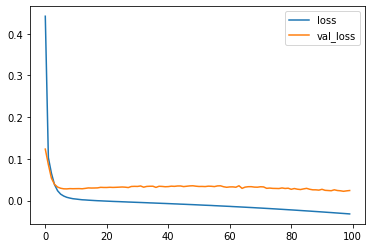
\includegraphics[width=.4\linewidth]{fig/loss.png}
		\label{fig:loss}}
	\subfigure[Accuracy]{\centering
		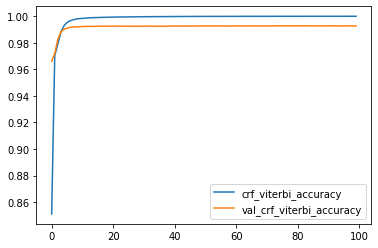
\includegraphics[width=.4\linewidth]{fig/acc.png}
		\label{fig:acc}}
	\caption{\label{fig:demo} Training curves of the bidirectional LSTM and CRF model trained for 100 epochs on the CoNLL-2003 dataset}
\end{figure}

\section{Lab NER}
The goal of the notebook is to implement a Named Entity Recognition (NER) system using bidirectional LSTMs and Conditional Random Fields (CRFs). For this task, the CoNLL-2003 dataset is used. A dataset that was specifically designed for language-independent NER. It consists of $\approx 300'000$ words and eight tags. The first few steps include loading the dataset and getting it into a format that can easily be used for model training. One of these steps includes padding, which is necessary because not all the sequences have the same length. Thus a max length is defined, and all shorter sequences will be padded. The model consists of an Input, Masking, Embedding and Bidirectional-LSTM layer. For the embedding layer, GloVe is used with either 100 or 300 dimensions. The model is then trained using CRF, which helps to predict sequences and not predict each token independently. The model was trained for 100 epochs. After every third epoch, the model was evaluated on the test set by printing the classification report that includes the precision, recall and f1-score.

Evaluating it on the test set here makes not much sense, in my opinion, since we have a validation set that we could use for that task. When using the test set for this task, we optimize the algorithm for it and lack generalization, for which the test set should be used as the last step. 

The model's loss and accuracy show that it converged, and it approached a validation accuracy of 99.3\%. However, when looking at the classification report, one can see that the model can recognize the tags present a lot in the dataset but lacks predicting the others (e.g. the beginning tags). Thus the macro averaged f1 score is only at 47\%.

\end{document}

